\documentclass[11pt]{article}
\usepackage[margin=1in]{geometry}
\usepackage{amsmath,amssymb,amsthm}
\usepackage{graphicx}
\usepackage[hidelinks]{hyperref}

\newtheorem{theorem}{Theorem}
\newtheorem{lemma}{Lemma}
\newtheorem{remark}{Remark}

\newcommand{\BFPP}{\mathrm{BFPP}}
\newcommand{\cf}{\operatorname{cf}}

\title{Compact ordered spaces and the ball fixed point property for \(C(K,p)\)}
\author{arXiv automatic math run \texttt{fa\_banach\_001}}
\date{2026-06-15}

\begin{document}
\maketitle

\section*{Source Question}

The source paper is Aviles--Japon--Lennard--Martinez-Cervantes--Stawski,
\emph{The ball fixed point property in spaces of continuous functions},
arXiv:2506.17995 \cite{source}.  It asks in final Question (i) whether there
exists an infinite compact space \(K\) and a non-isolated point \(p\in K\)
such that
\[
  C(K,p)=\{f\in C(K):f(p)=0\}
\]
has the ball fixed point property \(\BFPP\).

\begin{center}
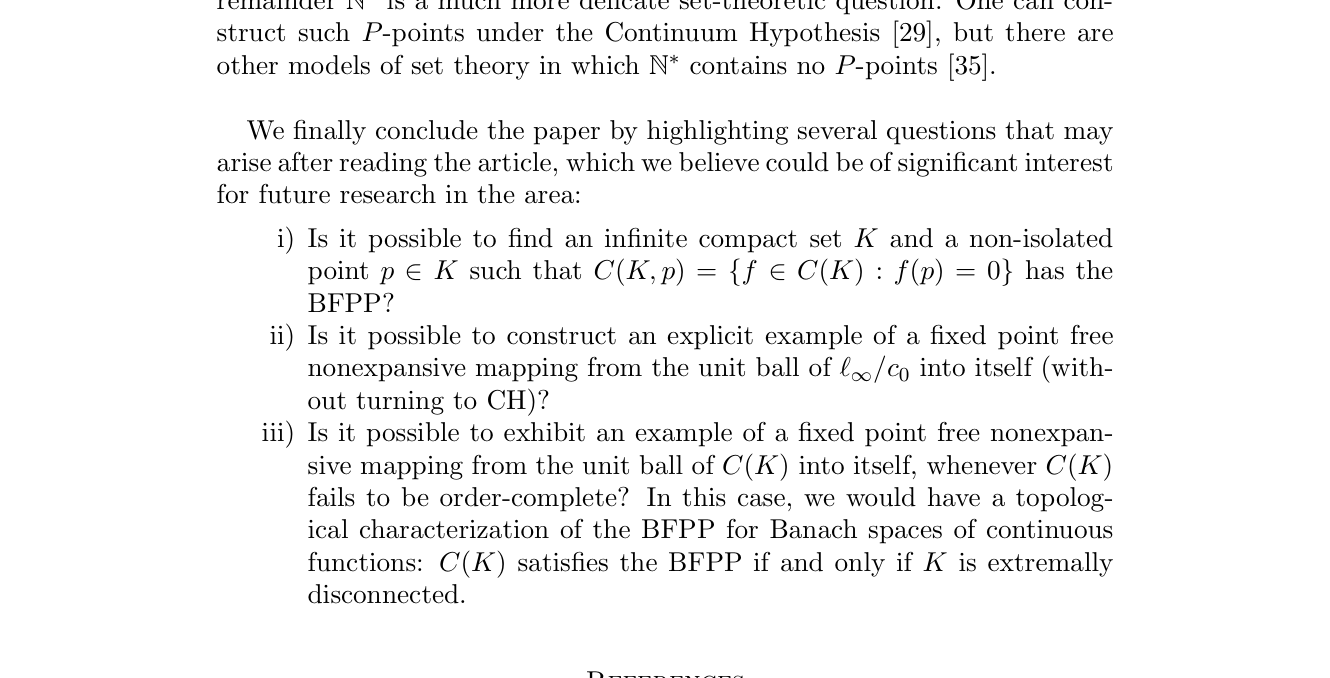
\includegraphics[width=\linewidth]{figures/open_question_i_crop.png}
\end{center}

The source paper proves failure when \(p\) is a non-\(P\)-point.  Previous
lane-15 packets proved failure for ordinal compacta and, more generally, for
points admitting a clopen ordinal tower.  This packet gives a different
extension: all compact linearly ordered spaces are negative examples.

\section*{Idea of the Proof}

Let \(K\) be a compact linearly ordered topological space and let \(p\) be
non-isolated.  From one side of \(p\) we can choose a closed subspace
\(F\subset K\) homeomorphic to an ordinal interval \([0,\kappa]\), with
\(\kappa\) a nonzero limit ordinal and \(p\) corresponding to \(\kappa\).  The
old ordinal shift gives a fixed-point-free nonexpansive self-map of the unit
ball of \(C(F,p)\).

The point of the ordered setting is that restriction to a closed ordered
subspace has a norm-one linear right inverse.  On each convex component of
\(K\setminus F\), extend a function on \(F\) by keeping it constant if the
component has only one boundary point in \(F\), and by interpolating between
the two boundary values if it has two.  This positive extension operator has
norm one and preserves the condition of vanishing at \(p\).  Therefore a bad
map on \(C(F,p)\) transfers to a bad map on \(C(K,p)\).

\section*{Ordered Extension Lemma}

\begin{lemma}\label{lem:extension}
Let \(K\) be a compact linearly ordered topological space and let \(F\subset K\)
be closed.  Then there is a positive linear operator
\[
  E:C(F)\longrightarrow C(K)
\]
with \(\|E\|=1\) and \(E f|_F=f\) for every \(f\in C(F)\).  Consequently, if
\(p\in F\), then \(E\) restricts to a norm-one linear right inverse
\[
  E:C(F,p)\longrightarrow C(K,p)
\]
for the restriction map \(R:C(K,p)\to C(F,p)\).
\end{lemma}

\begin{proof}
The components of \(K\setminus F\) are convex open intervals in the order.
For such a component \(I\), the boundary \(\overline I\setminus I\) is a
nonempty subset of \(F\) with either one or two points.  If it has one point
\(a\), put \((Ef)(x)=f(a)\) for \(x\in I\).  If it has two points \(a<b\),
choose, by normality of the compact interval \([a,b]\), a continuous function
\(\theta_I:[a,b]\to[0,1]\) such that \(\theta_I(a)=0\) and
\(\theta_I(b)=1\), and put
\[
  (Ef)(x)=(1-\theta_I(x))f(a)+\theta_I(x)f(b),\qquad x\in I.
\]
Finally set \((Ef)(x)=f(x)\) for \(x\in F\).

Linearity and positivity are immediate, and \(\|Ef\|_\infty\le\|f\|_\infty\)
because every value on a gap is a convex combination of boundary values.
Since \(E\) fixes \(F\), \(\|E\|=1\) when \(F\ne\emptyset\).

It remains only to note continuity at points of \(F\).  Let \(y\in F\) and
let \(x_i\to y\) be a net in \(K\).  If \(x_i\in F\) eventually, continuity
follows from that of \(f\).  Otherwise pass to points lying in components
\(I_i\) of \(K\setminus F\).  If a component \(I_i\) is adjacent to \(y\), then
the chosen interpolation tends to the boundary value \(f(y)\) as
\(x_i\to y\).  If \(I_i\) is not adjacent to \(y\), then its boundary points
in \(F\) eventually lie in every prescribed order-neighborhood of \(y\);
otherwise convexity would force the component to cross a fixed point of
\(F\) near \(y\).  The continuity of \(f\) on \(F\) then makes all boundary
values, and hence their convex combinations, converge to \(f(y)\).  Thus
\(Ef\in C(K)\).

If \(p\in F\) and \(f(p)=0\), then \(Ef(p)=f(p)=0\), so the same operator maps
\(C(F,p)\) into \(C(K,p)\).  It is a right inverse to restriction because it
fixes every point of \(F\).
\end{proof}

\section*{Ordinal Skeleton Lemma}

\begin{lemma}\label{lem:skeleton}
Let \(K\) be a compact linearly ordered topological space and let \(p\in K\)
be non-isolated.  Then there are a nonzero limit ordinal \(\kappa\) and a
closed \(F\subset K\) such that \(p\in F\) and \(F\) is homeomorphic to
\([0,\kappa]\), with \(p\) corresponding to \(\kappa\).
\end{lemma}

\begin{proof}
Since \(p\) is non-isolated, \(p\) is approached from at least one side.  We
write the proof for the case where \(p\) is in the closure of
\(\{x\in K:x<p\}\); the right-hand case is obtained by reversing the order.

Let \(\kappa=\cf(\{x\in K:x<p\})\), the cofinality of the initial segment
below \(p\).  Then \(\kappa\) is a nonzero limit ordinal.  Choose an increasing
cofinal family \((y_\alpha)_{\alpha<\kappa}\) below \(p\).  By transfinite
recursion, replacing it by a cofinal subsequence if necessary, choose a
strictly increasing continuous family \((x_\alpha)_{\alpha<\kappa}\) such that
\[
  x_\lambda=\sup_{\alpha<\lambda}x_\alpha
\]
for every nonzero limit \(\lambda<\kappa\), and
\(\sup_{\alpha<\kappa}x_\alpha=p\).  At a limit stage \(\lambda<\kappa\), the
supremum of the previous points is still below \(p\); otherwise the initial
segment below \(p\) would have cofinality at most \(\lambda<\kappa\).

Set
\[
  F=\{x_\alpha:\alpha<\kappa\}\cup\{p\}.
\]
The map \(x_\alpha\mapsto\alpha\), \(p\mapsto\kappa\), is a homeomorphism from
\(F\) onto \([0,\kappa]\): continuity at nonzero limit stages is exactly the
definition of \(x_\lambda\), and neighborhoods of \(p\) contain tails of the
cofinal family.  The same description shows that \(F\) contains all its order
limit points in \(K\), hence \(F\) is closed in \(K\).
\end{proof}

\section*{Partial Result}

\begin{lemma}\label{lem:ordinal}
Let \(\kappa\) be a nonzero limit ordinal.  Then
\[
  C([0,\kappa],\kappa)=\{f\in C([0,\kappa]):f(\kappa)=0\}
\]
fails \(\BFPP\).
\end{lemma}

\begin{proof}
Let \(X=C([0,\kappa],\kappa)\).  Define \(S:B_X\to B_X\) by
\[
(Sf)(\alpha)=
\begin{cases}
1, & \alpha=0,\\
f(\beta), & \alpha=\beta+1<\kappa,\\
f(\alpha), & 0<\alpha<\kappa \text{ is a limit ordinal},\\
0, & \alpha=\kappa.
\end{cases}
\]
The same successor-shift continuity check used for ordinal compacta shows
that \(Sf\in X\): at every limit ordinal the shifted successor values converge
to the already prescribed limit value of \(f\), and at \(\kappa\) they
converge to \(f(\kappa)=0\).  The map is nonexpansive because each coordinate
of \(Sf-Sg\) is either \(0\) or a coordinate of \(f-g\).

If \(f=Sf\), then \(f(0)=1\), and transfinite induction gives
\(f(\alpha)=1\) for every \(\alpha<\kappa\): the successor step follows from
\(f(\beta+1)=f(\beta)\), and the limit step follows from continuity.  This
contradicts \(f(\kappa)=0\).  Hence \(S\) is fixed-point-free.
\end{proof}

\begin{theorem}\label{thm:lots}
Let \(K\) be an infinite compact linearly ordered topological space and let
\(p\in K\) be non-isolated.  Then \(C(K,p)\) fails the ball fixed point
property.
\end{theorem}

\begin{proof}
By Lemma~\ref{lem:skeleton}, choose a closed \(F\subset K\), a nonzero limit
ordinal \(\kappa\), and a homeomorphism \(F\cong[0,\kappa]\) carrying \(p\) to
\(\kappa\).  By Lemma~\ref{lem:ordinal}, \(C(F,p)\) fails \(\BFPP\).
Equivalently, there is a fixed-point-free nonexpansive map
\[
  S:B_{C(F,p)}\longrightarrow B_{C(F,p)} .
\]

Let \(R:C(K,p)\to C(F,p)\) be restriction.  By Lemma~\ref{lem:extension},
there is a norm-one linear operator \(E:C(F,p)\to C(K,p)\) with \(R E\) equal
to the identity on \(C(F,p)\).  Define
\[
  T:B_{C(K,p)}\longrightarrow B_{C(K,p)},\qquad T(f)=E(S(Rf)).
\]
Since \(R\), \(S\), and \(E\) are all nonexpansive on the relevant unit balls,
\(T\) is nonexpansive and maps the unit ball of \(C(K,p)\) into itself.

If \(f\in B_{C(K,p)}\) were a fixed point of \(T\), then applying \(R\) would
give
\[
  Rf = R E S Rf = S(Rf),
\]
contradicting that \(S\) is fixed-point-free.  Hence \(T\) is a
fixed-point-free nonexpansive self-map of the closed unit ball of \(C(K,p)\),
so \(C(K,p)\) fails \(\BFPP\).
\end{proof}

\section*{Scope and Limitations}

This result extends the ordinal compact packet to all compact ordered spaces.
It includes connected compact intervals and long-line type compacta, where a
clopen-tower argument is not available.  The result is still a partial answer
to the source question: arbitrary compact Hausdorff spaces need not contain a
closed one-sided ordinal skeleton with a norm-one extension operator.

\section*{Novelty and Verification Notes}

The local run indexes were searched for arXiv \texttt{2506.17995}, BFPP,
\(C(K,p)\), ordered compacta, LOTS, and extension-operator language.  No prior
packet for compact linearly ordered spaces was found.  A bounded web search on
2026-06-15 for exact combinations of \(C(K,p)\), BFPP, and linearly ordered
compact spaces found no later explicit answer to this subcase.

Human review should focus on Lemma~\ref{lem:extension}, especially continuity
of the interpolation extension at points of \(F\) which are limits of many
convex gaps.  Once that lemma is accepted, the transfer of the ordinal
fixed-point-free map is formal.

\begin{thebibliography}{9}
\bibitem{source}
A. Aviles, M. Japon, C. Lennard, G. Martinez-Cervantes, A. Stawski,
\emph{The ball fixed point property in spaces of continuous functions},
arXiv:2506.17995, 2025.
\end{thebibliography}

\end{document}
